% ============================================================================
\section{State-space models}
% ============================================================================

\begin{frame}[t]{Attention's cost, and the recurrent alternative}
  \begin{itemize}\itemsep0.45em
    \item Everything in this deck so far keeps attention and makes it cheaper. This section covers the one thread that asks a different question: does the sequence mixer have to be attention at all?
    \item The motivation is the KV cache from earlier. Attention keeps every past token individually addressable, which is exactly why it can retrieve anything, and exactly why serving memory grows with context and batch size.
    \item A recurrence trades the other way: history is compressed into a fixed-size state $h_t$, so a decoding step costs the same no matter how much context precedes it. 2017-era RNNs had that property, but they trained sequentially and lost long-range detail.
    \item The state-space line asks for both at once: a constant-size state \emph{and} training that is parallel across the sequence. (Shrinking or paging the cache is the other answer to the same problem, and is covered later in the course.)
  \end{itemize}
\end{frame}

\begin{frame}[t]{S4: a structured linear recurrence}
  \begin{itemize}\itemsep0.15em
    \item Start from a continuous linear system $h'(t) = Ah(t) + Bx(t)$, $y(t) = Ch(t)$ and discretize it with a step size $\Delta$: $h_t = \bar{A}h_{t-1} + \bar{B}x_t$, $y_t = Ch_t$. A linear RNN, with no nonlinearity in the state update.
    \item Because the parameters are the same at every position (linear time-invariant), unrolling gives a convolution $y = K * x$ with $K = (C\bar{B},\, C\bar{A}\bar{B},\, C\bar{A}^2\bar{B},\, \ldots)$: training is one global convolution instead of $L$ sequential steps.
    \item S4 makes that practical. Initialize $A$ from HiPPO theory so the state holds a compressed summary of the history, and parameterize it as diagonal-plus-low-rank so $K$ can be computed stably as a Cauchy kernel.
    \item It won on the regime transformers struggled with: state of the art on every Long Range Arena task, including the first solution of Path-X at length 16k.
    \item The limitation is inside ``time-invariant'': one fixed kernel applies to every token, so the model cannot keep or discard something because of what that token is.
  \end{itemize}
  {\scriptsize Gu et al., ``Efficiently Modeling Long Sequences with Structured State Spaces,'' \href{https://arxiv.org/abs/2111.00396v3}{arXiv:2111.00396v3}.}
\end{frame}

\begin{frame}[t]{Mamba: selection breaks time-invariance}
  \begin{itemize}\itemsep0.1em
    \item Mamba's one change: let $B$, $C$, and the discretization step $\Delta$ be functions of the current token. $A$ stays fixed, but $\Delta_t$ modulates it through the discretization, so the effective $\bar{A}_t$ and $\bar{B}_t$ now vary along the sequence.
    \item Read $\Delta_t$ as a gate. Large means reset the state toward the current token; small means ignore this token and hold what the state already has: content-based filtering inside a linear recurrence.
    \item The evidence is synthetic and sharp: time-invariant models solve copying at fixed spacing, but fail selective copying and induction heads, which require deciding what to keep from the content.
  \end{itemize}
  \centering
  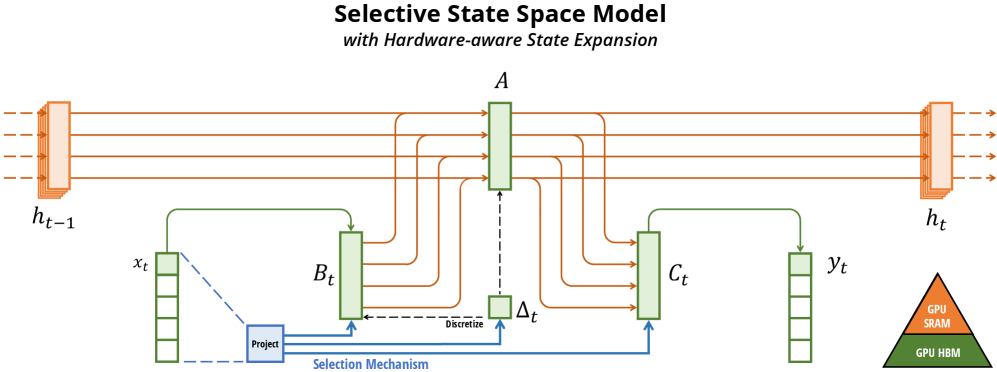
\includegraphics[width=0.92\textwidth,height=0.27\textheight,keepaspectratio]{images/transformers-2017-v-2026/mamba_paper_fig1_selective_ssm_overview.png}\\[0.1em]
  {\scriptsize Gu \& Dao, ``Mamba: Linear-Time Sequence Modeling with Selective State Spaces,'' \href{https://arxiv.org/abs/2312.00752v2}{arXiv:2312.00752v2}, Figure~1.}
\end{frame}

\begin{frame}[t]{The Mamba block and the parallel scan}
  \begin{itemize}\itemsep0.1em
    \item Selectivity costs the convolution: per-token parameters leave no single kernel, so the recurrence must be run. Mamba runs it as a \textbf{hardware-aware parallel scan} keeping the expanded state in SRAM and recomputing it in the backward pass instead of writing it to HBM, FlashAttention's argument applied to a recurrence.
    \item Cost model: training is linear in sequence length and still parallel; at inference the state is fixed size, so each step is $O(1)$ memory and $L$ tokens cost $O(L)$ time, with no cache that grows.
    \item Reported payoff: roughly 5$\times$ the generation throughput of a same-size Transformer, with Mamba-3B matching Transformers about twice its size.
  \end{itemize}
  \centering
  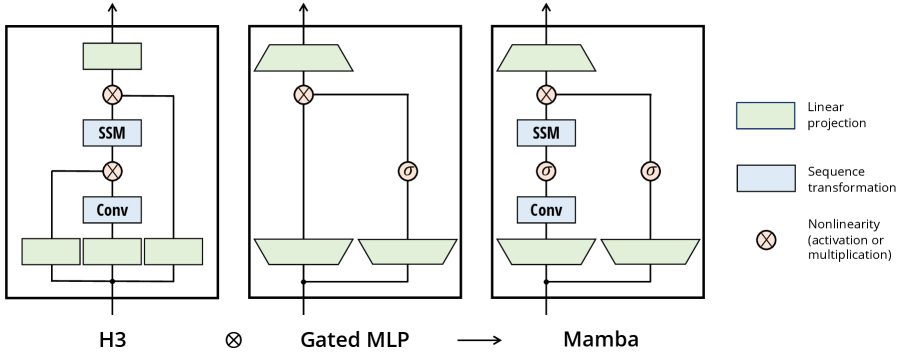
\includegraphics[width=0.70\textwidth,height=0.23\textheight,keepaspectratio]{images/transformers-2017-v-2026/mamba_paper_fig3_block_architecture.png}\\[0.1em]
  {\scriptsize The block folds H3 (an earlier attention-free SSM layer) and a gated MLP into one unit. Gu \& Dao, \href{https://arxiv.org/abs/2312.00752v2}{arXiv:2312.00752v2}, Figure~3.}
\end{frame}

\begin{frame}[t]{Mamba-2: state-space duality}
  \begin{columns}[T,onlytextwidth]
    \column{0.66\textwidth}
    \begin{itemize}\itemsep0.35em
      \item Write a linear SSM's whole sequence map as one matrix, $y = Mx$. That $M$ is \textbf{semiseparable}: its off-diagonal blocks are low rank.
      \item Multiplying by $M$ as a recurrence is linear in $L$; materializing it and applying it row by row is a masked-attention form, quadratic in $L$. Structured state-space duality says these are two algorithms for one computation, not two model families.
      \item Mamba-2 cashes that in: restricting $A$ to a scalar times the identity lets the layer run as large matmuls on tensor cores, 2--8$\times$ faster than Mamba's selective scan and with a far larger state.
      \item So the efficient-attention thread and the SSM thread met in the middle. Linear attention, gated recurrences, and selective SSMs are one design space.
    \end{itemize}

    \column{0.32\textwidth}
    \centering
    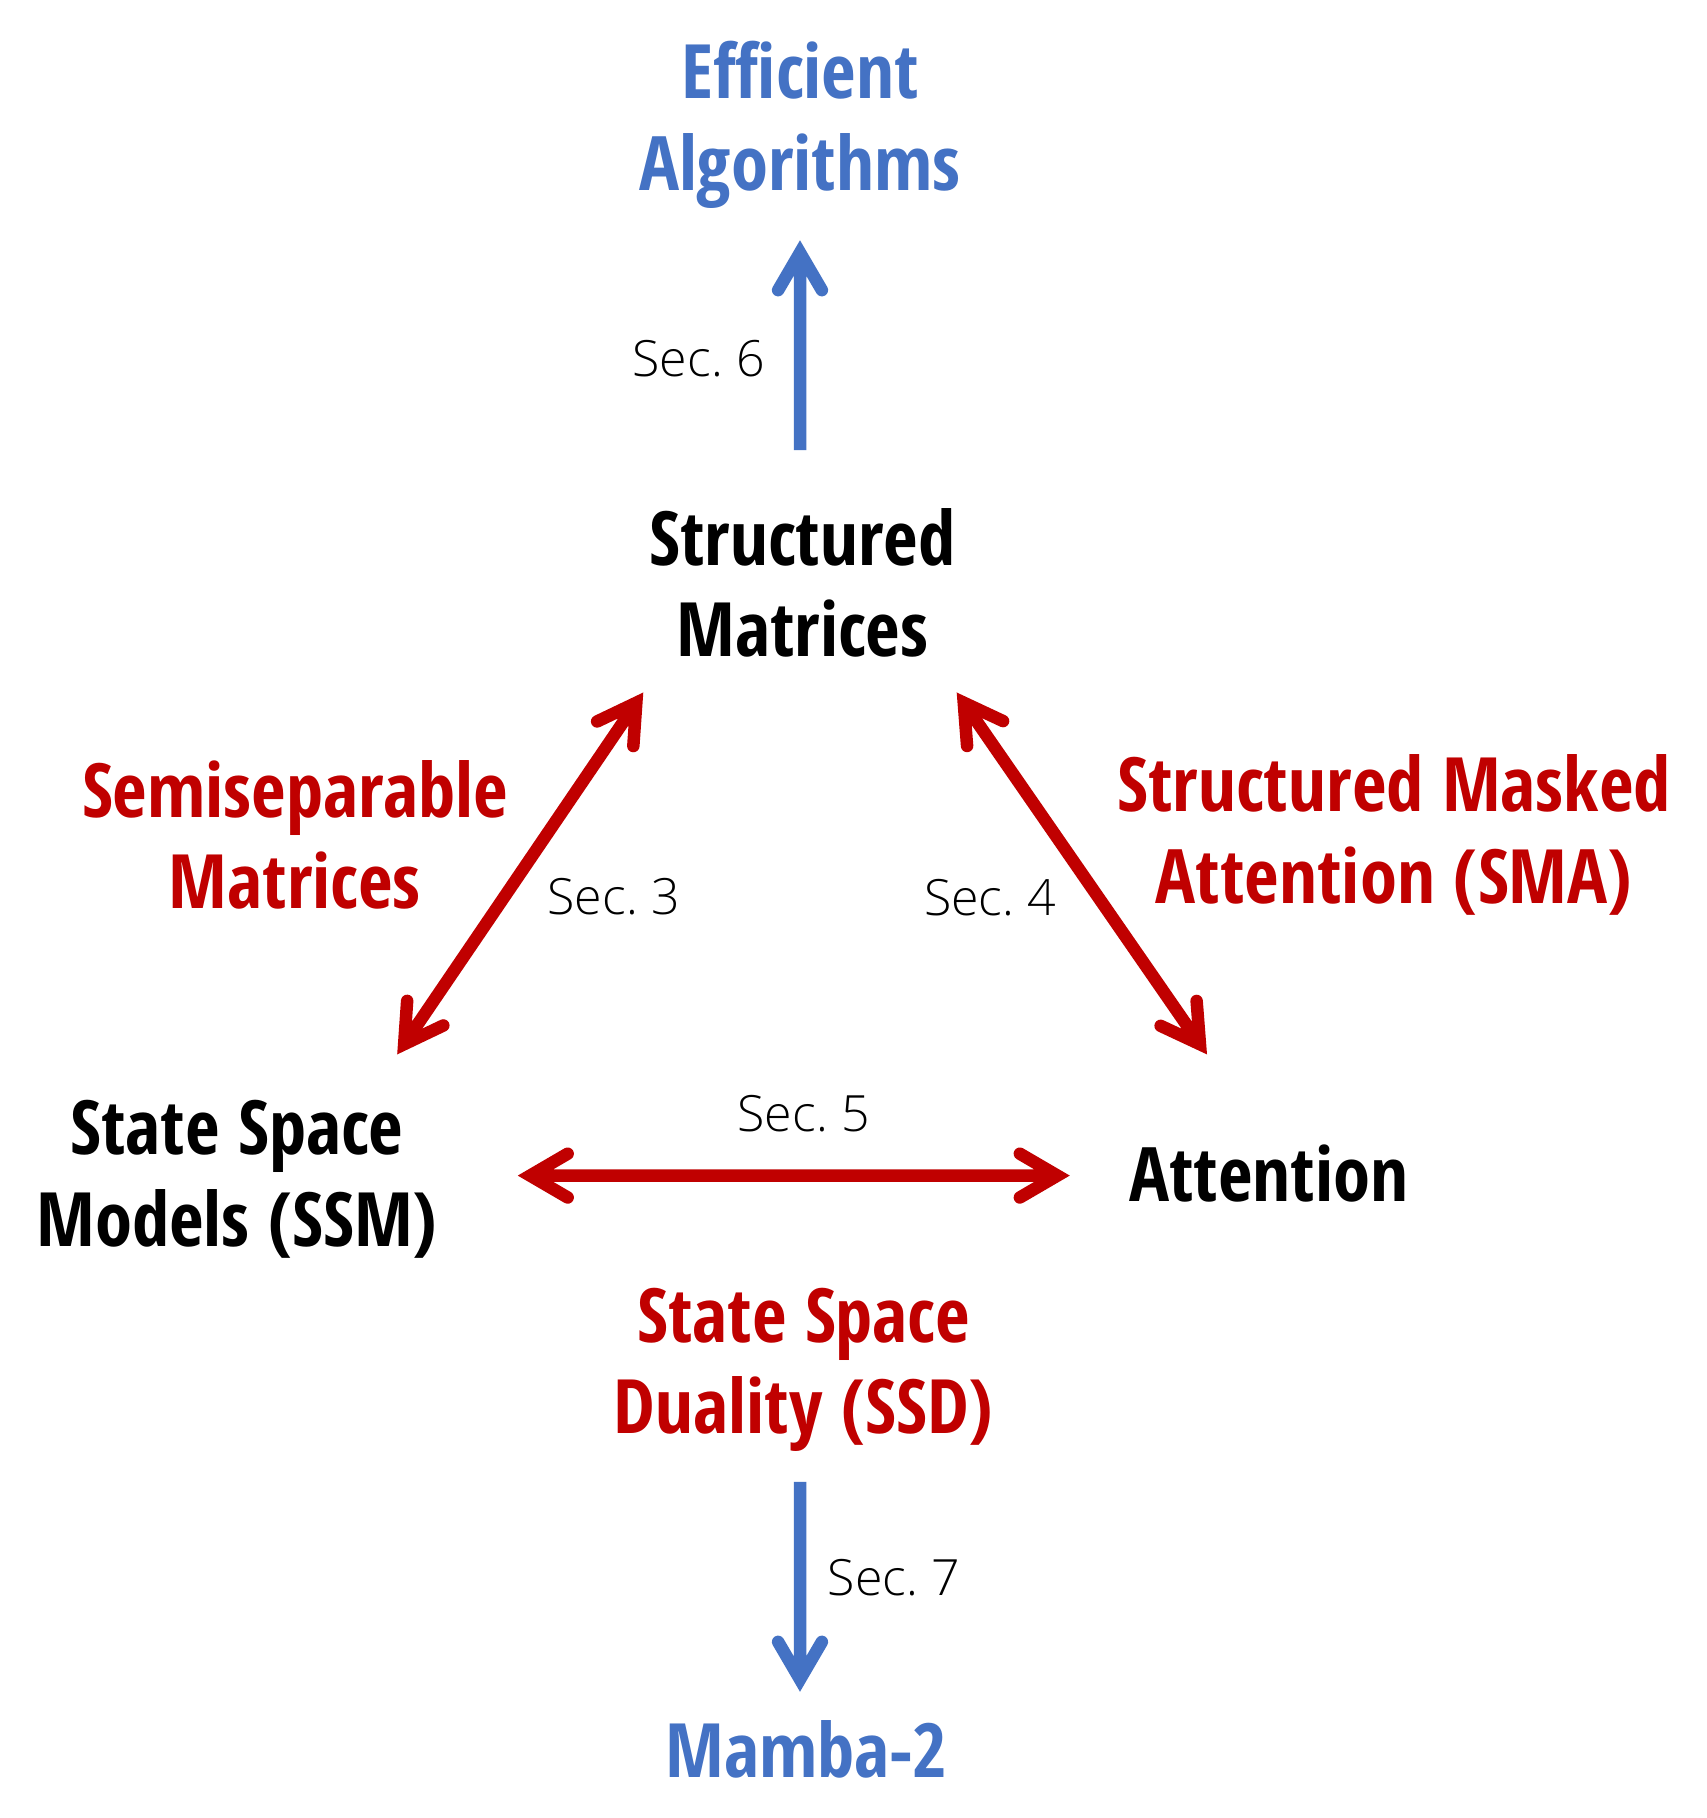
\includegraphics[width=\linewidth,height=0.55\textheight,keepaspectratio]{images/transformers-2017-v-2026/mamba2_ssd_fig1_duality_roadmap.png}\\[0.15em]
    {\scriptsize Dao \& Gu, ``Transformers are SSMs,'' \href{https://arxiv.org/abs/2405.21060v1}{arXiv:2405.21060v1}, Figure~1.}
  \end{columns}
\end{frame}

\begin{frame}[t]{Hybrids: Jamba, Griffin, and after}
  \begin{columns}[T,onlytextwidth]
    \column{0.64\textwidth}
    \begin{itemize}\itemsep0.15em
      \item \textbf{Jamba} (2024) interleaves Mamba layers, Transformer layers, and MoE. Its blocks are $l = 8$ layers at a 1:7 attention-to-Mamba ratio, with MoE every second layer: 52B total, 12B active, 256K context.
      \item The number that explains the design: at 256K tokens the KV cache is 4\,GB, against 32\,GB for Mixtral, because only the attention layers keep one.
      \item \textbf{Griffin} (2024) swaps the SSM for a real-gated linear recurrent unit interleaved with local sliding-window attention. Hawk (pure recurrence) exceeds Mamba's reported results; Griffin matches Llama-2 on 6$\times$ fewer tokens.
      \item By 2025 hybrids are the shipping form, the sliding-window recipe with a cheaper layer type: Zamba2, Nemotron-H, Falcon-H1, RecurrentGemma.
    \end{itemize}

    \column{0.34\textwidth}
    \centering
    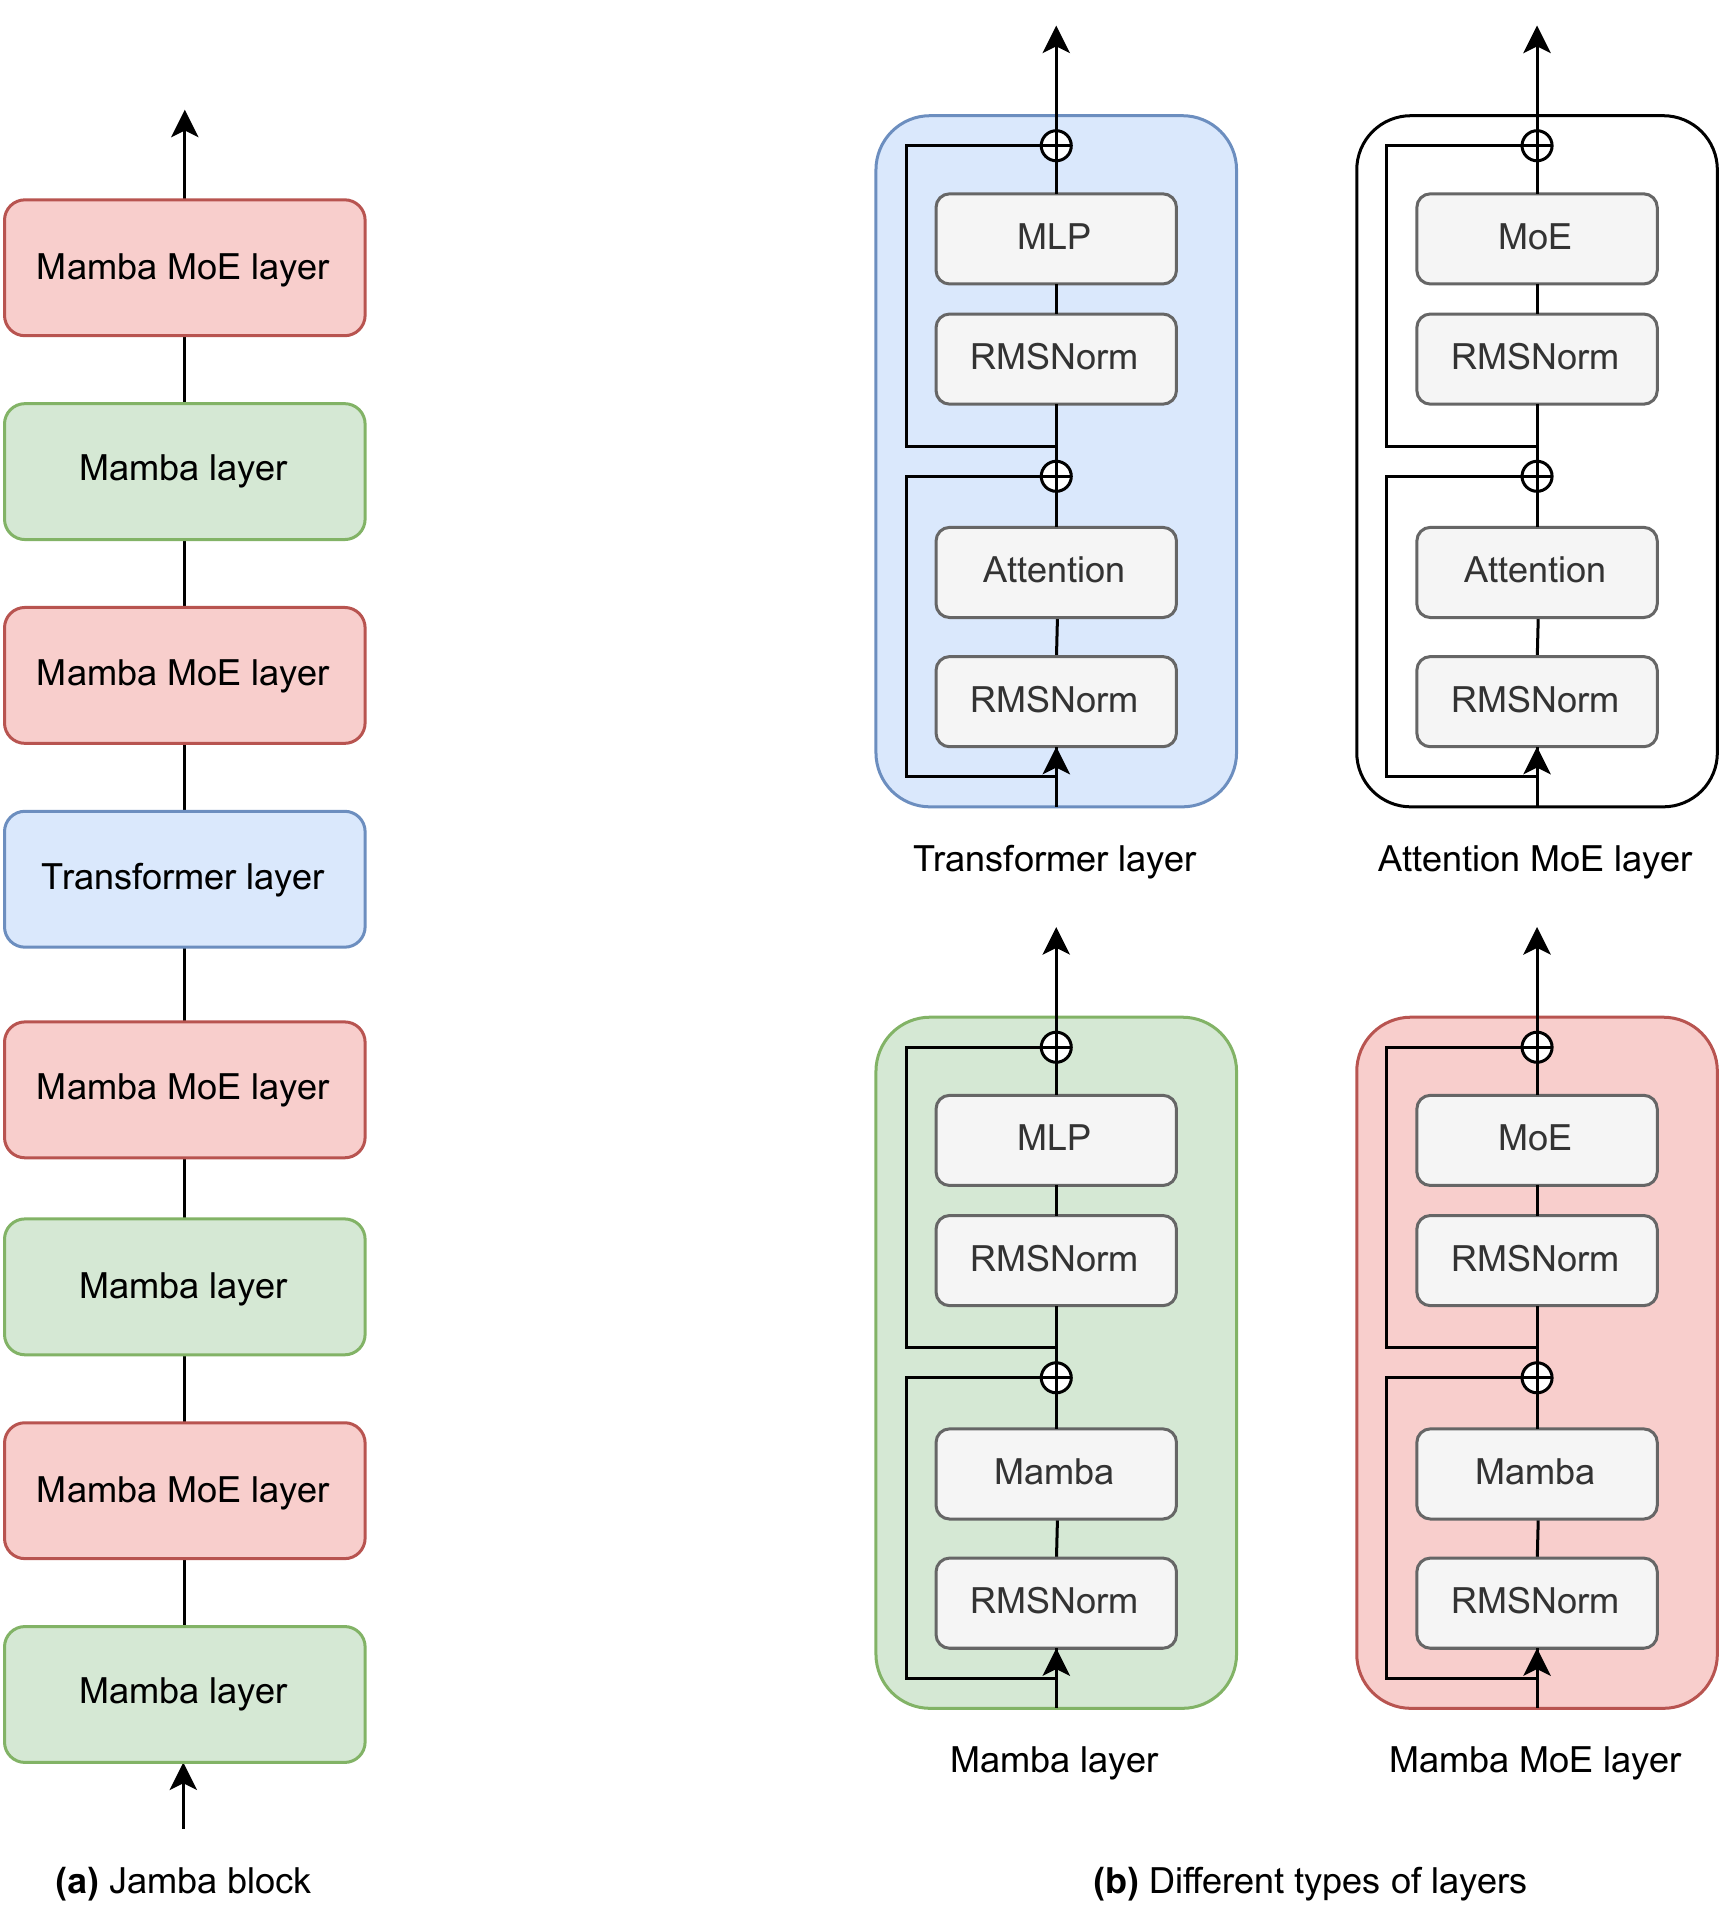
\includegraphics[width=\linewidth,height=0.58\textheight,keepaspectratio]{images/transformers-2017-v-2026/jamba_paper_fig1_block_and_layer_types.png}\\[0.15em]
    {\scriptsize Lieber et al., ``Jamba: A Hybrid Transformer-Mamba Language Model,'' \href{https://arxiv.org/abs/2403.19887v1}{arXiv:2403.19887v1}, Figure~1.}
  \end{columns}
\end{frame}

\begin{frame}[t]{Scorecard: what a fixed state costs}
  \begin{itemize}\itemsep0.4em
    \item A fixed-size state is a summary, and whatever the summary dropped is gone. Attention keeps every token addressable, and pays memory for that exact recall.
    \item ``Repeat After Me'' makes it concrete: any fixed-state model provably fails to copy strings carrying more bits than its state holds, and empirically Transformers learn copying from far fewer samples, generalize to longer strings, and beat same-size Mamba at in-context lookup even where Mamba has the lower perplexity.
    \item Jamba's own ablation agrees. At 1.3B, pure Mamba scores 48.8 on IMDB against 84.1 for pure attention, often failing to produce the answer format at all; the hybrid recovers it at 90.9. The authors read this as weak in-context learning, tied to the absence of induction heads.
    \item The wins are real but narrower than the headlines: throughput and memory at long context, streaming inference, and modalities such as audio and genomics.
  \end{itemize}
\end{frame}

\begin{frame}{Copying and lookup: Transformers vs.\ SSMs}
  \centering
  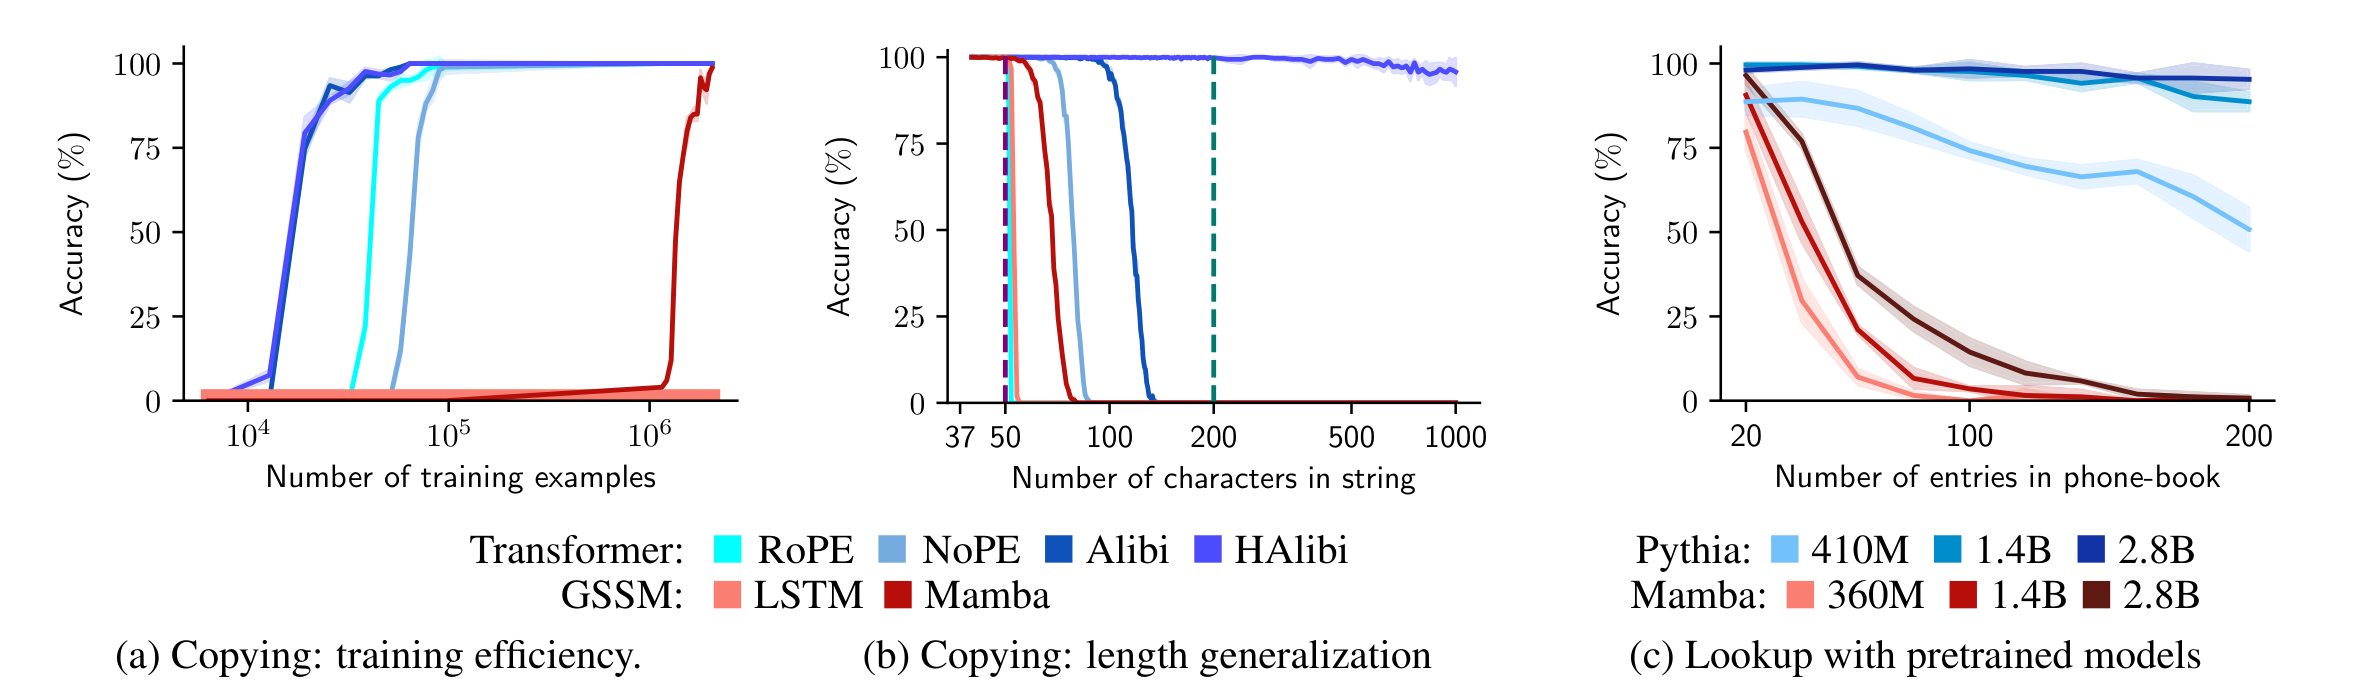
\includegraphics[width=\textwidth,height=0.66\textheight,keepaspectratio]{images/transformers-2017-v-2026/repeat_after_me_fig1_copying_and_lookup.png}\\[0.3em]
  {\scriptsize Transformers (blues) against fixed-state models (reds) on copying and retrieval. (a) sample efficiency when learning to copy; (b) accuracy on strings longer than those seen in training, with the training length and context window marked; (c) pretrained Pythia against pretrained Mamba at comparable sizes, retrieving a number from an in-context phone book. \textit{Reference:} Jelassi et al., ``Repeat After Me: Transformers are Better than State Space Models at Copying,'' \href{https://arxiv.org/abs/2402.01032v2}{arXiv:2402.01032v2}, Figure~1.}
\end{frame}

\begin{frame}[t]{Verdict (2026)}
  \begin{itemize}\itemsep0.45em
    \item Attention was not replaced. What survived from this thread is a layer type, not an architecture: SSM and gated-recurrence layers carry most of the depth, and a handful of attention layers keep exact retrieval available.
    \item That is the same economics as the sliding-window hybrids earlier in this deck. Make the common layer cheap in memory traffic, then pay for a few expensive layers where the capability actually lives.
    \item Structured state-space duality dissolved the border between the two research programs, so ``attention versus SSM'' now reads better as a choice of mixing matrix inside one family.
    \item Which is this deck's recurring lesson once more: the changes that stuck are the ones that move less memory per token. Byte-level and diffusion language models change the tokenizer and decoding order rather than the mixer; both come later in the course.
  \end{itemize}
\end{frame}
